\documentclass[12pt]{article}

%%%%%%%%%%%%%%%%%%%%%%%%%%%%%%%%%%%%%%%%%%%%%%%%%%%%%%%%%%%%%%%%%%%%%%%%%%%%%%%%%%%%%%%%%%%%%%%%%%%%
% Math
\usepackage{fancyhdr} 
\usepackage{amsfonts}
\usepackage{amsmath}
\usepackage{amssymb}
\usepackage{amsthm}
%\usepackage{dsfont}

%%%%%%%%%%%%%%%%%%%%%%%%%%%%%%%%%%%%%%%%%%%%%%%%%%%%%%%%%%%%%%%%%%%%%%%%%%%%%%%%%%%%%%%%%%%%%%%%%%%%
% Macros
\usepackage{calc}

%%%%%%%%%%%%%%%%%%%%%%%%%%%%%%%%%%%%%%%%%%%%%%%%%%%%%%%%%%%%%%%%%%%%%%%%%%%%%%%%%%%%%%%%%%%%%%%%%%%%
% Commands and Custom Variables	
\newcommand{\problem}[1]{\hspace{-4 ex} \large \textbf{Problem #1} }
%\let\oldemptyset\emptyset
%\let\emptyset\varnothing
\newcommand{\norm}[1]{\left\lVert#1\right\rVert}
\newcommand{\sint}{\text{s}\kern-5pt\int}
\newcommand{\powerset}{\mathcal{P}}
\renewenvironment{proof}{\hspace{-4 ex} \emph{Proof}:}{\qed}
\newcommand{\solution}{\textit{Solution}:\bigbreak}
\newcommand{\RR}{\mathbb{R}}
\newcommand{\NN}{\mathbb{N}}
\newcommand{\QQ}{\mathbb{Q}}
\newcommand{\ZZ}{\mathbb{Z}}
\newcommand{\CC}{\mathbb{C}}
\newcommand{\VV}{\mathbb{V}}
\newcommand{\FF}{\mathbb{F}}
\renewcommand{\Re}{\operatorname{Re}}
\renewcommand{\Im}{\operatorname{Im}}

\newcommand{\bigO}{\mathcal{O}}

\renewcommand{\vec}[1]{\boldsymbol{\mathbf{#1}}}

\newcommand{\editnote}[1]{\textcolor{red}{\textbf{\MakeUppercase{#1}}}}


%%%%%%%%%%%%%%%%%%%%%%%%%%%%%%%%%%%%%%%%%%%%%%%%%%%%%%%%%%%%%%%%%%%%%%%%%%%%%%%%%%%%%%%%%%%%%%%%%%%%
%page
\usepackage[margin=1in]{geometry}
\usepackage{setspace}
%\doublespacing
\allowdisplaybreaks
\pagestyle{fancy}
\fancyhf{}
\rhead{Shaw \space \thepage}
\setlength\parindent{0pt}
\usepackage{color}

%%%%%%%%%%%%%%%%%%%%%%%%%%%%%%%%%%%%%%%%%%%%%%%%%%%%%%%%%%%%%%%%%%%%%%%%%%%%%%%%%%%%%%%%%%%%%%%%%%%%
%Code
\usepackage{listings}
\usepackage{courier}
\lstset{
	language=Python,
	showstringspaces=false,
	formfeed=newpage,
	tabsize=4,
	commentstyle=\itshape,
	basicstyle=\ttfamily,
}

%%%%%%%%%%%%%%%%%%%%%%%%%%%%%%%%%%%%%%%%%%%%%%%%%%%%%%%%%%%%%%%%%%%%%%%%%%%%%%%%%%%%%%%%%%%%%%%%%%%%
%Images
\usepackage{graphicx}
\graphicspath{ {images/} }
\usepackage{float}

%tikz
\usepackage[utf8]{inputenc}
%\usepackage{pgfplots}
%\usepgfplotslibrary{groupplots}

%%%%%%%%%%%%%%%%%%%%%%%%%%%%%%%%%%%%%%%%%%%%%%%%%%%%%%%%%%%%%%%%%%%%%%%%%%%%%%%%%%%%%%%%%%%%%%%%%%%%
%Hyperlinks
%\usepackage{hyperref}
%\hypersetup{
%	colorlinks=true,
%	linkcolor=blue,
%	filecolor=magenta,      
%	urlcolor=cyan,
%}

\begin{document}
	\thispagestyle{empty}
	
	\begin{flushright}
		Sage Shaw \\
		m567 - Fall 2018 \\
		\today
	\end{flushright}
	
\begin{center}{\large \textbf{Homework 2}}\end{center}
\bigbreak

\hspace{-.5 ex}\problem{1} 

\textit{Lemma}: Given two vectors $\vec{a}, \vec{x} \in \CC^N$ the product of their circulants is the circulant of their convolution. That is
$$
\text{circ}(\vec{a})\text{circ}(\vec{x}) = \text{circ}(\text{conv}(\vec{a}, \vec{b}))
$$

\begin{proof}
	Let for any vector $\vec{v} \in \CC^N$ define $v_{-j} = v_{N-j}$ and $v_{j+N} = v_j$ for $j=0, 1, 2, \dots, N-1$. Then the convolution of two vectors $\vec{a}, \vec{x} \in \CC^N$ is given element-wise by
	$$
	\text{conv}(\vec{a}, \vec{x})_m = \sum\limits_{j=0}^{N-1} a_{m-j}x_j, \ \ m=0,1,\dots, N-1 \text{.}
	$$
	For a given vector the circulant is defined element-wise by
	$$
	\text{circ}(\vec{a})_{ij} = a_{i-j}, \ \ \ i,j=0,1,\dots, N-1\text{.}
	$$
	Let $\vec{a},\vec{x} \in \CC^N$. Then
	\begin{align*}
		\big( \text{circ}(\vec{a}) \text{circ}(\vec{x}) \big)_{ij} &= \sum\limits_{k=0}^{N-1} \text{circ}(\vec{a})_{ik} \text{circ}(\vec{x})_{kj} \\
		&= \sum\limits_{k=0}^{N-1} a_{i-k} x_{k-j} \text{.}
	\end{align*}
	Also
	\begin{align*}
	\text{circ}(\text{conv}(\vec{a}, \vec{x}))_{ij} &= \sum\limits_{k=0}^{N-1} a_{(i-j)-k}x_k \\
	&= \sum\limits_{k=0}^{N-1} a_{i-(k+j)}x_k \\
	&= \sum\limits_{l=j}^{N-1+j} a_{i-l}x_{l-j} \\
	&= \sum\limits_{l=0}^{N-1} a_{i-l}x_{l-j}
	\end{align*}
\end{proof}

We are now ready to prove the theorem.\bigbreak

\begin{proof}
	Let $\vec{a}, \vec{x} \in \CC^N$, and define
	\begin{align*}
		\vec{b} &= \text{conv}(\vec{a},\vec{x}) &&\\
		A &= \text{circ}(\vec{a}) & \hat{A} &= \text{diag}(\hat{\vec{a}}) \\
		X &= \text{circ}(\vec{x}) & \hat{X} &= \text{diag}(\hat{\vec{x}}) \\
		B &= \text{circ}(\vec{v}) & \hat{B} &= \text{diag}(\hat{\vec{b}}) \text{.}
	\end{align*}
	%define $A = \text{circ}(\vec{a})$, $X = \text{circ}(\vec{x})$, $\hat{A} = \text{diag}(\hat{\vec{a}})$, and $\vec{b} = A\vec{x}$. 
	Further define $\omega_N = e^{\frac{2\pi}{N}\mathbf{i}}$ and the matrix $U$ by $U_{ij} = \omega_N^{ij}$. Then $U^{-1} = \frac{1}{N}U^{*}$ and 
	\begin{align*}
	(AU)_{mn} &= \sum\limits_{i=0}^{N-1}a_{m-i}\omega_N^{in} \\
	&= \sum\limits_{k=m}^{N-1+m}a_{k}\omega_N^{(m-k)n} \\
	&= \sum\limits_{k=0}^{N-1}a_{k}\omega_N^{(m-k)n} \\
	\frac{1}{N}(U^{*}AU)_{ln} &= \frac{1}{N} \sum\limits_{m=0}^{N-1} \omega_N^{-lm} \left( \sum\limits_{k=0}^{N-1}a_{k}\omega_N^{(m-k)n} \right) \\
	&= \frac{1}{N} \sum\limits_{m=0}^{N-1}\sum\limits_{k=0}^{N-1} \omega_N^{-lm + (m-k)n} a_{k} \\
	&= \frac{1}{N} \sum\limits_{m=0}^{N-1}\sum\limits_{k=0}^{N-1} \omega_N^{(n-l)m -nk} a_{k} \\
	&= \sum\limits_{m=0}^{N-1} \omega_N^{(n-l)m} \frac{1}{N} \sum\limits_{k=0}^{N-1} a_{k}\omega_N^{-nk}  \\
	& = \sum\limits_{m=0}^{N-1} \omega_N^{(n-l)m} \hat{a}_k \\
	& = \begin{cases} N \hat{a}_k & \text{ if } l=n \\
					0 & \text{ else}
		\end{cases} \\
	&= \hat{A}_{ln} \text{.}
	\end{align*}
	Note that by the previous lemma, $AX = B$, and consider
	\begin{align*}
		\hat{A}\hat{X} & = \frac{1}{N}U^{*}AU \frac{1}{N}U^{*}XU \\
		& = \frac{1}{N}U^{*}AXU \\
		& = \frac{1}{N}U^{*}BU \\
		& = \hat{B} \text{.}
	\end{align*}
	Let $\vec{1}$ denote a vector of length $N$ of all ones. Then
	\begin{align*}
	\hat{A}\hat{X} \vec{1} &= \hat{B} \vec{1} \\
	\hat{A}\hat{\vec{x}} &= \hat{\vec{b}} \text{.}
	\end{align*}
\end{proof}

\bigbreak
%%%%%%%%%%%%%%%%%%%%%%%%%%%%%%%%%%%%%%%%%%%%%%%%%%%%%%%%%%%%%%%%%%%%%%%%%%%%%%%%%%%%%%%%%%%%%%%%%%%%
\problem{2(a)} The following function calculates the product $A\vec{x}$ where $A$ is a Toeplitz matrix, and $\vec{x}$ is a vector, using the FFT.
\begin{lstlisting}[language=Python]
def toep_mult(A, x):
	N = len(x)
	a = np.block([A[:,0], A[0,:0:-1]] )
	a_hat = fft.fft(a)
	x_hat = fft.fft(np.block([x, np.zeros(N-1)]))
	b_hat = a_hat * x_hat # Scipy's FFT isn't scaled
	b = fft.ifft(b_hat)
	return b[:N]
\end{lstlisting}



%%%%%%%%%%%%%%%%%%%%%%%%%%%%%%%%%%%%%%%%%%%%%%%%%%%%%%%%%%%%%%%%%%%%%%%%%%%%%%%%%%%%%%%%%%%%%%%%%%%%
\problem{2(b)} The following code test the function above for the Toeplitz matrix provided on 100 random vectors of lengths $N= 10, 100, 500, 1000, \text{ and }5000$. 
\begin{lstlisting}[language=Python]
Ns = [10, 100, 500, 1000, 5000]
times = 100
errs = []
for N in Ns:
	my_errs = []
	A = toeplitz([1/i for i in range(1,N+1)], 
			[-1/i for i in range(1,N+1)]).T
			#The syntax of the toeplitz function in scipy
			#uses the first element of the column for the
			#main diagonal this transpose is done to eusure 
			#the main diagonal is 1 instead of -1
	for i in range(times):
		x = np.random.randn(N)
		err = np.max(np.abs(A@x - toep_mult(A,x)))
		my_errs.append(err)
	errs.append(my_errs)
my_maxs = np.max(errs, axis=1)
my_mins = np.min(errs, axis=1)
my_ave  = np.mean(errs, axis=1)
\end{lstlisting}

The $L^\infty$ errors can be seen in the following table.
\begin{center}
	\begin{tabular}{|c|c|c|c|}
		\hline
		$N$&Min $L^\infty$ Error&Average $L^\infty$ Error&Max $L^\infty$ Error\\ \hline
		10&1.1102e-15&3.751e-15&7.9936e-15\\ \hline
		100&3.5705e-13&6.1594e-13&1.005e-12\\ \hline
		500&6.4525e-15&9.2852e-15&1.3512e-14\\ \hline
		1000&4.3194e-11&5.1539e-11&7.6112e-11\\ \hline
		5000&9.6812e-14&1.1659e-13&1.5099e-13\\ \hline
	\end{tabular}
\end{center}
These results verify that the multiplication is done correctly. It is interesting to see that the error is much higher for $N=1000$. To explore this further, errors were calculated for all integer values between $N=900$ and $N=1099$ and graphed in the plot below. It's worth noting that there are many $N$ for which the error gets as high as $10^{-10}$, but that for any given $N$ the maximum error and the minimum error are within an order of magnitude. This suggests that the larger error is due to the size of the vector and not due to the randomness. It is unclear weather this is inherent to the method, the hardware, or to SciPy's implementation of FFT functions.

\begin{figure}[H]
	%\caption{Equispaced points}
	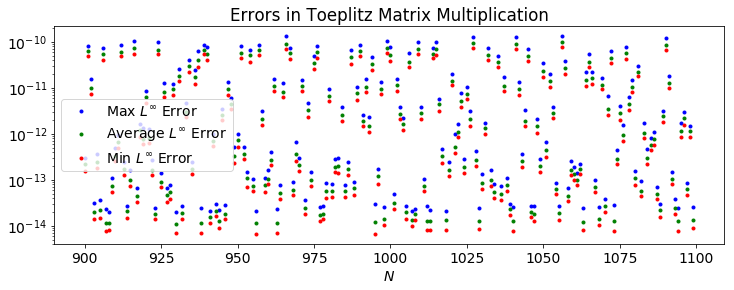
\includegraphics[width=1\textwidth]{hw02_p2_b_toeplitz_mult_errors}
	\centering
\end{figure}

\bigbreak

%%%%%%%%%%%%%%%%%%%%%%%%%%%%%%%%%%%%%%%%%%%%%%%%%%%%%%%%%%%%%%%%%%%%%%%%%%%%%%%%%%%%%%%%%%%%%%%%%%%%
\problem{3(a)} Consider the $N$ by $N$ system $A \vec{u} = \vec{f}$, where $A$ is symmetric and tridiagonal with constant $b$ on the main diagonal and constant $a$ on the subdiagonal/superdiagonal. Let $\hat{u}$ and $\hat{f}$, denote the discrete sine transforms of $\vec{u}$ and $\vec{f}$ respectively. Then for $j = 1, ..., N-1$ we have the equation
\begin{align*}
	2\sum\limits_{k=1}^{N-1} \hat{f}_{j} \sin \left(\tfrac{\pi jk}{N}\right) &= a2\sum\limits_{k=1}^{N-1} \hat{u}_{k} \sin \left(\tfrac{\pi (j-1)k}{N}\right) + b2 \sum\limits_{k=1}^{N-1} \hat{u}_k \sin \left(\tfrac{\pi jk}{N} \right)  \\
	&\phantom{===} + a2\sum\limits_{k=1}^{N-1} \hat{u}_{k} \sin \left(\tfrac{\pi (j+1)k}{N} \right) \\
	& = \sum\limits_{k=1}^{N-1} \hat{u}_{k} \left( 2a \sin \left(\tfrac{\pi (j-1)k}{N}\right) + 2a \sin \left(\tfrac{\pi (j+1)k}{N}\right)  + 2b \sin \left(\tfrac{\pi jk}{N} \right) \right) \\
	& = \sum\limits_{k=1}^{N-1} \hat{u}_{k} \left( 2a \left( 2\sin \left(\tfrac{\pi jk}{N}\right) \cos \left(\tfrac{\pi k}{N}\right) \right) + 2b \sin \left(\tfrac{\pi jk}{N} \right) \right) \\
	& = 2 \sum\limits_{k=1}^{N-1} \hat{u}_{k} \left( 2a\cos \left(\tfrac{\pi k}{N}\right) +b \right) \sin \left(\tfrac{\pi jk}{N}\right)\\
	\sum\limits_{k=1}^{N-1} \hat{f}_{j} \sin \left(\tfrac{\pi jk}{N}\right) &= \sum\limits_{k=1}^{N-1} \hat{u}_{k} \left( 2a\cos \left(\tfrac{\pi k}{N}\right) +b \right) \sin \left(\tfrac{\pi jk}{N}\right) \text{.}
\end{align*}

\bigbreak

%%%%%%%%%%%%%%%%%%%%%%%%%%%%%%%%%%%%%%%%%%%%%%%%%%%%%%%%%%%%%%%%%%%%%%%%%%%%%%%%%%%%%%%%%%%%%%%%%%%%
\problem{3(b)} Notice that the result at the end of the last section can be expressed more compactly as
$$
\text{iDST}(\hat{\vec{f}}) = \text{iDST}\left( \left(2a\cos \tfrac{\pi \vec{k}}{N} +b\right) \hat{\vec{u}} \right)
$$
and since the iDST is invertible, we can equate the vectors $\hat{f}_k = \left(2a\cos \tfrac{\pi k}{N} +b\right) \hat{u}_k$. Rearanging the terms we arrive at
$$
\hat{u}_k = \frac{\hat{f}_k}{2a\cos \tfrac{\pi k}{N} +b}, \ \ \ k=1,\dots, N-1
$$
as desired.

\bigbreak
%%%%%%%%%%%%%%%%%%%%%%%%%%%%%%%%%%%%%%%%%%%%%%%%%%%%%%%%%%%%%%%%%%%%%%%%%%%%%%%%%%%%%%%%%%%%%%%%%%%%
\problem{3(c)} These steps can be combined into the following algorithm
\begin{enumerate}
	\item calculate $\hat{\vec{f}}$ via the DST of $\vec{f}$
	\item calculate $\hat{\vec{u}}$ by $\hat{\vec{u}}_k = \frac{\hat{\vec{f}}_k}{2a \cos \left(\frac{\pi k}{N} \right) + b}$
	\item calculate $\vec{u}$ via the inverse DST of $\hat{\vec{u}}$
\end{enumerate}
This algorithm is implemented in the code below.
\begin{lstlisting}[language=Python]
def fast_tri_diag(a, b, fs):
	n = len(fs)
	f_hat = fft.dst(fs,type=1)/(2*n+2)
	u_hat = f_hat / (2*a * np.cos(
np.pi*np.arange(1,n+1)/(n+1)) + b)
	return fft.idst(u_hat, type=1)
\end{lstlisting}

\bigbreak

%%%%%%%%%%%%%%%%%%%%%%%%%%%%%%%%%%%%%%%%%%%%%%%%%%%%%%%%%%%%%%%%%%%%%%%%%%%%%%%%%%%%%%%%%%%%%%%%%%%%
\problem{3(d)} This was applied to the problem
$$
u''(x) = \tanh(4\sin(x)), \ \ 0 \leq x \leq \pi, \ \  u(0)=u(\pi) = 0
$$
for $N$= 100, and the resulting solution is plotted below.
\begin{figure}[H]
	%\caption{Equispaced points}
	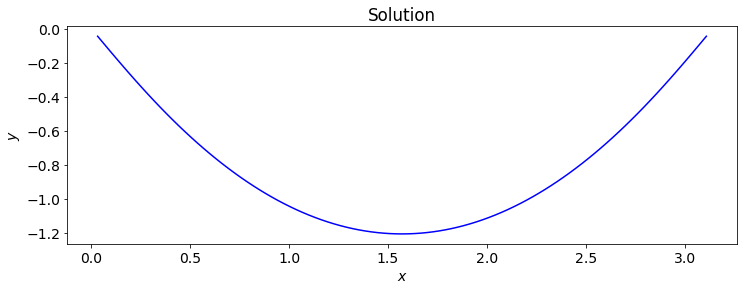
\includegraphics[width=1\textwidth]{hw02_p3d_plot}
	\centering
\end{figure}



\bigbreak

%%%%%%%%%%%%%%%%%%%%%%%%%%%%%%%%%%%%%%%%%%%%%%%%%%%%%%%%%%%%%%%%%%%%%%%%%%%%%%%%%%%%%%%%%%%%%%%%%%%%
\problem{4(a)} To derive the implicit FD formula for the Helmholtz equation
$$
u''(x) + k^2 u(x) = f(x), a\leq x \leq b
$$
we will need the following formulae: \\
\textit{second order approximation to the second derivative}
$$
\frac{1}{h^2}\begin{bmatrix} 0 & 1 & -2 & 1 & 0 \end{bmatrix}\vec{u} = \vec{u}'' + \bigO(h^2)
$$
\textit{fourth order approximation to the second derivative}
$$
\frac{1}{12h^2}\begin{bmatrix} -1 & 16 & -30 & 16 & -1 \end{bmatrix}\vec{u} = \vec{u}'' + \bigO(h^4)
$$
\textit{second order approximation to the fourth derivative}
$$
\frac{1}{h^4}\begin{bmatrix} 1 & -4 & 6 & -4 & 1 \end{bmatrix}\vec{u} = \vec{u}^{(4)} + \bigO(h^2) 
$$

Applying our fourth order approximation we have that
\begin{align}
	\vec{f} + \bigO(h^4) &= \frac{1}{12h^2}\begin{bmatrix} -1 & 16 & -30 & 16 & -1 \end{bmatrix}\vec{u} + k^2 \vec{u} \nonumber \\
	\frac{12}{12}\vec{f} + \bigO(h^4)&= \frac{1}{12h^2}\begin{bmatrix} -1 & 16 & (12h^2k^2-30) & 16 & -1 \end{bmatrix}\vec{u}\text{.} \label{like_equ9}
\end{align}
Differentiating the Helmholtz equation twice and applying our second order approximations to $u^{(4)}, u'',$ and $f''$ we have
\begin{align}
 \frac{1}{h^2}\begin{bmatrix} 1 & -2 & 1 \end{bmatrix}\vec{f} + \bigO(h^2) &= \frac{1}{h^4}\begin{bmatrix} 1 & -4 & 6 & -4 & 1 \end{bmatrix}\vec{u} +  \frac{k^2}{h^2}\begin{bmatrix} 0 & 1 & -2 & 1 & 0 \end{bmatrix}\vec{u} \nonumber \\
&= \frac{1}{h^4}\begin{bmatrix} 1 & -4 & 6 & -4 & 1 \end{bmatrix}\vec{u} \nonumber \\
	& \phantom{===} +   \frac{h^2k^2}{h^4}\begin{bmatrix} 0 & 1 & -2 & 1 & 0 \end{bmatrix}\vec{u} \nonumber \\
&= \frac{1}{h^4}\begin{bmatrix} 1 & (h^2k^2-4) & (6-2h^2k^2) & (h^2k^2-4) & -1 \end{bmatrix}\vec{u}\text{.} \label{like_equ10}
\end{align}
%\frac{1}{h^2}\begin{bmatrix} 1 & -2 & 1 \end{bmatrix}
Summing $(\ref{like_equ9}) + \frac{h^2}{12} (\ref{like_equ10})$ we have
\begin{align*}
	\frac{1}{12}\begin{bmatrix} 1 & 10 & 1 \end{bmatrix}\vec{f} + \bigO(h^4) &= \begin{bmatrix} (k^2+\frac{12}{h^2}) & (10k^2-\frac{24}{h^2}) & (k^2+\frac{12}{h^2})\end{bmatrix}\vec{u}
\end{align*}
a fourth order three point stencil for the Helmholtz equation. It remains to calculate the stencils for the boundary. When accounting for the boundaries we arrive at the following system
$$
D\vec{u} = E\vec{f} + \left[f_0 - \alpha(k^2+\tfrac{12}{h^2}) \right] \vec{e}_1 + \left[f_{n+1} - \beta(k^2+\tfrac{12}{h^2}) \right] \vec{e}_{n}
$$
where $f_0=f(a), f_{n+1}=f(b), \alpha = u(a), \text{ and }\beta=u(b)$. 

%De note the appropriate values at the boundaries as follows.
%\begin{align*}
%	x&=a & \alpha &= u(a) & f_0&=f(a) \\
%	x&=b & \beta &= u(b) & f_{n+1}&=f(b)
%\end{align*}
%Then the stencils for the boundaries are given by
%$\begin{align*}
%	\frac{1}{12} + \bigO(h^4) &= \begin{bmatrix} (k^2+\frac{12}{h^2}) & (10k^2-\frac{24}{h^2}) & (k^2+\frac{12}{h^2})\end{bmatrix}\vec{u}
%\end{align*}



%The five point fourth order accurate stencil for the approximation to the second derivative is given as
%\begin{align*}
%	\frac{1}{12h^2}\begin{bmatrix} -1 & 16 & -30 & 16 & -1 \end{bmatrix}\vec{u} = \vec{u}'' + \bigO(h^4)\text{.}
%\end{align*}
%The second order accurate approximation to the fourth derivative is given as
%\begin{align*}
%\frac{1}{h^4}\begin{bmatrix} 1 & -4 & 6 & -4 & 1 \end{bmatrix}\vec{u} = \vec{u}^{(4)} + \bigO(h^2) \text{.}
%\end{align*}
%substituting these into the Helmholtz equation $u''(x) + k^2 u(x) = f(x), a\leq x \leq b$, and the equation given by differentiating both sides $u^{(4)}(x) + k^2 u''(x) = f''(x), a\leq x \leq b$ we have the following equations:
%\begin{align}
% \frac{1}{12h^2}\begin{bmatrix} -1 & 16 & 12h^2k^2-30 & 16 & -1 \end{bmatrix}\vec{u} &= \vec{f} + \bigO(h^4)\\
% \frac{1}{h^4}\begin{bmatrix} 1 & h^2k^2-4 & 6-2h^2k^2-4 & h^2k^2-4-4 & 1 \end{bmatrix}\vec{u} &= \frac{1}{h^2}\begin{bmatrix} 1 & -2 & 1 \end{bmatrix}\vec{f} + \bigO(h^2) \\
%\end{align}

\bigbreak

%%%%%%%%%%%%%%%%%%%%%%%%%%%%%%%%%%%%%%%%%%%%%%%%%%%%%%%%%%%%%%%%%%%%%%%%%%%%%%%%%%%%%%%%%%%%%%%%%%%%
\problem{4(b)} Given particular the Helmholtz equation
$$
u''(x) + 150^2u(x) = 1, 0 \leq x \leq 1
$$
with the boundary conditions of $u(0)=1$ and $u(1)=0$ for which the exact solution is
$$
u(x) = \frac{1}{k^2} + \left(1 - \frac{1}{k^2} \right)\cos(kx) - \left( \frac{1}{k^2} + \left( 1 - \frac{1}{k^2}\right) \cos(k)\right) \csc(k) \sin(kx) \text{,}
$$
we can find a fourth order approximate solution by using the implicit formula from part (a).
\begin{lstlisting}[language=Python]
a, b = 0, 1
alpha, beta = 1, 0
f0, f_last = 1, 1
k = 150
n = 2**17 - 1

h = 1/(n+1)

h2 = h**2
k2 = k**2

xs = np.linspace(a+h, b-h, n)

#D = sp.diags([[12/h2+k2]*(n-1), [10*k2-24/h2]*n, 
		[12/h2+k2]*(n-1) ], offsets=[-1, 0, 1], format='csr')
E = sp.diags([[1]*(n-1), [10]*n, [1]*(n-1)], 
		offsets=[-1, 0, 1], format='csr')

fs = E@np.ones(n)
fs[0] += f0 - (12/h2+k2)*alpha
fs[-1] += f_last - (12/h2+k2)*beta

#us = spla.spsolve(D, fs)
us = fast_tri_diag(12/h2+k2, 10*k2-24/h2, fs)
\end{lstlisting}
\bigbreak

Below is the plot of our solution for the most accurate grid where $h = 2^{-15}$.
\begin{figure}[H]
	%\caption{Equispaced points}
	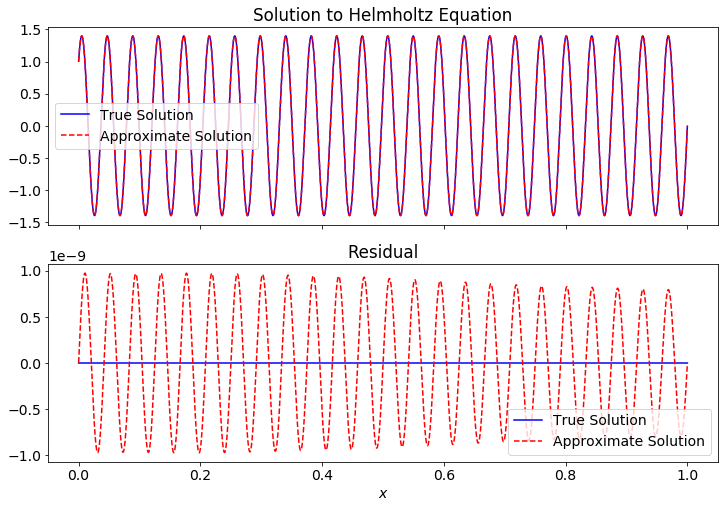
\includegraphics[width=1\textwidth]{hw02_p4a_solution}
	\centering
\end{figure}

As seen in the plot below, the order of convergence is roughly $\bigO(h^4)$. 
\begin{figure}[H]
	%\caption{Equispaced points}
	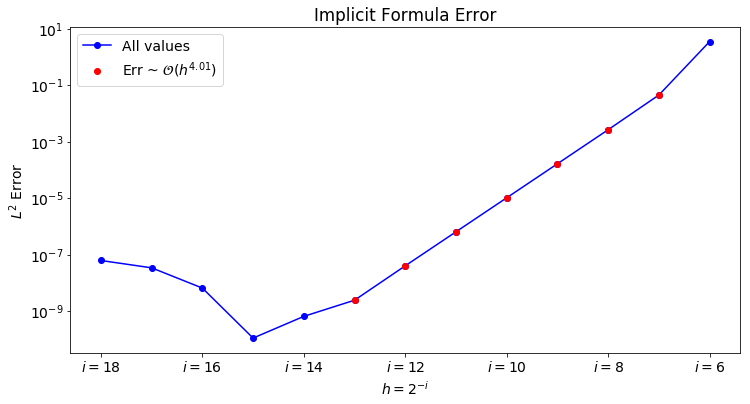
\includegraphics[width=1\textwidth]{hw02_p4a_convergence_2}
	\centering
\end{figure}

I haven't decided, but at the moment I prefer my error plots to be vs $N$ instead of $h$.

\begin{figure}[H]
	%\caption{Equispaced points}
	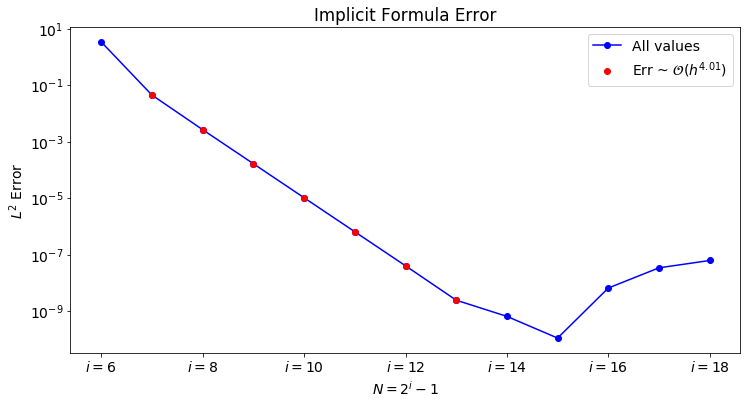
\includegraphics[width=1\textwidth]{hw02_p4a_convergence}
	\centering
\end{figure}


\bigbreak



\end{document}
